\begin{frame}{$\DPLL$ algorithms}

    $\varphi \coloneqq (x \lor \neg{y} \land z) \land (\neg{x} \lor w \land z \land s) \land
    (\neg{x} \lor \neg{z} \lor s) \land \dots$

    \pause
    \begin{center}
    	\begin{frame}

    \begin{center}
        \Huge Part II: SAT Solving and Proof Complexity
    \end{center}
    
\end{frame}

\begin{frame}{$\DPLL$ Algorithms}

    \begin{center}
        \begin{frame}

    \begin{center}
        \Huge Part II: SAT Solving and Proof Complexity
    \end{center}
    
\end{frame}

\begin{frame}{$\DPLL$ Algorithms}

    \begin{center}
        \begin{frame}

    \begin{center}
        \Huge Part II: SAT Solving and Proof Complexity
    \end{center}
    
\end{frame}

\begin{frame}{$\DPLL$ Algorithms}

    \begin{center}
        \input{pics/dpll.tex}        
    \end{center}

    
	\pause
    \pause
    \pause
    \pause
    \pause
    \begin{itemize}
        \item Heuristic $\mathbf{A}$ chooses a variable for splitting.
    	\pause
	    \item Heuristic $\mathbf{B}$ chooses the first value.
    	\pause
    	\item Simplification rules: \alert{no simplifications!}
    \end{itemize}
\end{frame}

\begin{frame}{$\DPLL$ and Resolution}
    
    \begin{theorem}
        $\DPLL$ algoritm makes $t$ splitting on \alert{unsatisfiable} CNF formula
        $$\varphi \coloneqq \bigwedge\limits_i C_i$$
        $\Rightarrow$ there exists a resolution proof of $\varphi$ of size $2t$.
    \end{theorem}

    \pause

    \begin{minipage}{0.58\linewidth}
        \centering
        \input{pics/dpll-2.tex}
    \end{minipage}
    \pause
    \begin{minipage}{0.4\linewidth}
        \centering
        $\frac{A \lor x ~~~ B \lor \neg x}{A \lor B} ~~~~~ \frac{A}{A \lor z}$
        \begin{itemize}
            \item Node $\Rightarrow$ disjunction of negations of queries.
            \item $(x \lor \neg y \lor \neg z \lor u)$.
        \end{itemize}
    \end{minipage}

\end{frame}

\begin{frame}{Corollaries}

    \begin{itemize}
        \item{} Running time of $\DPLL$ on $\PHP_{n}^{n + 1}$ is at least $2^{\Omega(n)}$.
            \pause
        \item{} [Alekhnovich, Hirsch, Itsykson 05; \alert{informal}] Running time of \alert{restricted}
            $\DPLL$ on some \alert{sat. formulas} is at least $2^{\Omega(n)}$. 
    \end{itemize}

    \pause
    \vspace{0.5cm}
    \begin{block}{Remark}
        $\alg{CDCL} \approx$ general resolution.
    \end{block}

    \pause
    \begin{itemize}
        \item{} Running time of $\alg{CDCL}$ on $\PHP_{n}^{n + 1}$ is at least $2^{\Omega(n)}$.
        \item{} \alert{Open problem}: what about sat. formulas and $\alg{CDCL}$?
    \end{itemize}

\end{frame}
        
    \end{center}

    
	\pause
    \pause
    \pause
    \pause
    \pause
    \begin{itemize}
        \item Heuristic $\mathbf{A}$ chooses a variable for splitting.
    	\pause
	    \item Heuristic $\mathbf{B}$ chooses the first value.
    	\pause
    	\item Simplification rules: \alert{no simplifications!}
    \end{itemize}
\end{frame}

\begin{frame}{$\DPLL$ and Resolution}
    
    \begin{theorem}
        $\DPLL$ algoritm makes $t$ splitting on \alert{unsatisfiable} CNF formula
        $$\varphi \coloneqq \bigwedge\limits_i C_i$$
        $\Rightarrow$ there exists a resolution proof of $\varphi$ of size $2t$.
    \end{theorem}

    \pause

    \begin{minipage}{0.58\linewidth}
        \centering
        \tikzstyle{inner} = [circle, minimum size = 0.3cm, draw, inner sep = 0.1pt]
\tikzstyle{gstyle} = [fill = green]
\tikzstyle{rstyle} = [fill = red]
\tikzstyle{ed} = [->, draw]
\tikzstyle{ops} = [alt=<{#1-}>{opacity = 1}{opacity = 0}]
\tikzstyle{opstyle} = [inner, ops = #1]
\tikzstyle{oped} = [ed, ops = #1]
\tikzstyle{gstyle} = [alt=<{#1}>{fill = green}{}]
\tikzstyle{rstyle} = [alt=<{#1}>{red!90!black}{}]
\tikzstyle{snakestyle} = [
    alt=<{#1}>{
        decorate,
        decoration = {
            snake,
            amplitude = 0.4mm,
            segment length = 2mm,
            post length = 1mm
        }
    }{}]


    
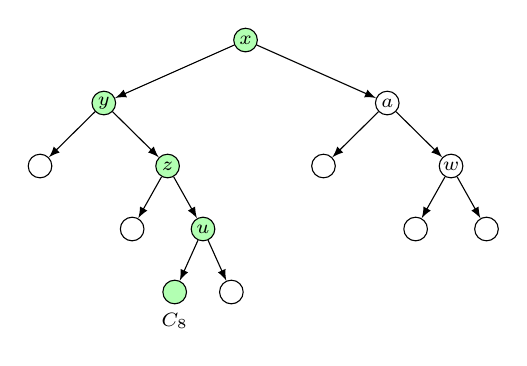
\begin{tikzpicture}[>=latex, xscale = 0.9]
    
    \node[inner, fill = green!30] (a) at (0, 0) {\scriptsize $x$};
    \node[inner, fill = green!30] (b) at (-2, -0.8) {\scriptsize $y$};
    \node[inner] (c) at (2, -0.8) {\scriptsize $a$};
    \node[inner] (d) at (-2.9, -1.6) {};
    \node[inner, fill = green!30] (e) at (-1.1, -1.6) {\scriptsize $z$};
    \node[inner] (f) at (1.1, -1.6) {};
    \node[inner] (g) at (2.9, -1.6) {\scriptsize $w$};

    \node[inner] (h) at (-1.6, -2.4) {};
	\node[inner, fill = green!30] (i) at (-0.6, -2.4) {\scriptsize $u$};
    
    \node[inner] (j) at (2.4, -2.4) {};
    \node[inner] (k) at (3.4, -2.4) {};

    \node[inner, fill = green!30] (l) at (-1, -3.2) {};
    \node[below = 4pt] at (l) {\scriptsize $C_{8}$};
    \node[inner] (m) at (-0.2, -3.2) {};
    
    \draw[ed] (a) -- (b);
    \draw[ed] (a) -- (c);
    \draw[ed] (b) -- (d);
    \draw[ed] (b) -- (e);
    \draw[ed] (c) -- (f);
    \draw[ed] (c) -- (g);
    \draw[ed] (e) -- (h);
    \draw[ed] (e) -- (i);
    \draw[ed] (g) -- (j);
    \draw[ed] (g) -- (k);
    \draw[ed] (i) -- (l);
    \draw[ed] (i) -- (m);
\end{tikzpicture}
    \end{minipage}
    \pause
    \begin{minipage}{0.4\linewidth}
        \centering
        $\frac{A \lor x ~~~ B \lor \neg x}{A \lor B} ~~~~~ \frac{A}{A \lor z}$
        \begin{itemize}
            \item Node $\Rightarrow$ disjunction of negations of queries.
            \item $(x \lor \neg y \lor \neg z \lor u)$.
        \end{itemize}
    \end{minipage}

\end{frame}

\begin{frame}{Corollaries}

    \begin{itemize}
        \item{} Running time of $\DPLL$ on $\PHP_{n}^{n + 1}$ is at least $2^{\Omega(n)}$.
            \pause
        \item{} [Alekhnovich, Hirsch, Itsykson 05; \alert{informal}] Running time of \alert{restricted}
            $\DPLL$ on some \alert{sat. formulas} is at least $2^{\Omega(n)}$. 
    \end{itemize}

    \pause
    \vspace{0.5cm}
    \begin{block}{Remark}
        $\alg{CDCL} \approx$ general resolution.
    \end{block}

    \pause
    \begin{itemize}
        \item{} Running time of $\alg{CDCL}$ on $\PHP_{n}^{n + 1}$ is at least $2^{\Omega(n)}$.
        \item{} \alert{Open problem}: what about sat. formulas and $\alg{CDCL}$?
    \end{itemize}

\end{frame}
        
    \end{center}

    
	\pause
    \pause
    \pause
    \pause
    \pause
    \begin{itemize}
        \item Heuristic $\mathbf{A}$ chooses a variable for splitting.
    	\pause
	    \item Heuristic $\mathbf{B}$ chooses the first value.
    	\pause
    	\item Simplification rules: \alert{no simplifications!}
    \end{itemize}
\end{frame}

\begin{frame}{$\DPLL$ and Resolution}
    
    \begin{theorem}
        $\DPLL$ algoritm makes $t$ splitting on \alert{unsatisfiable} CNF formula
        $$\varphi \coloneqq \bigwedge\limits_i C_i$$
        $\Rightarrow$ there exists a resolution proof of $\varphi$ of size $2t$.
    \end{theorem}

    \pause

    \begin{minipage}{0.58\linewidth}
        \centering
        \tikzstyle{inner} = [circle, minimum size = 0.3cm, draw, inner sep = 0.1pt]
\tikzstyle{gstyle} = [fill = green]
\tikzstyle{rstyle} = [fill = red]
\tikzstyle{ed} = [->, draw]
\tikzstyle{ops} = [alt=<{#1-}>{opacity = 1}{opacity = 0}]
\tikzstyle{opstyle} = [inner, ops = #1]
\tikzstyle{oped} = [ed, ops = #1]
\tikzstyle{gstyle} = [alt=<{#1}>{fill = green}{}]
\tikzstyle{rstyle} = [alt=<{#1}>{red!90!black}{}]
\tikzstyle{snakestyle} = [
    alt=<{#1}>{
        decorate,
        decoration = {
            snake,
            amplitude = 0.4mm,
            segment length = 2mm,
            post length = 1mm
        }
    }{}]


    
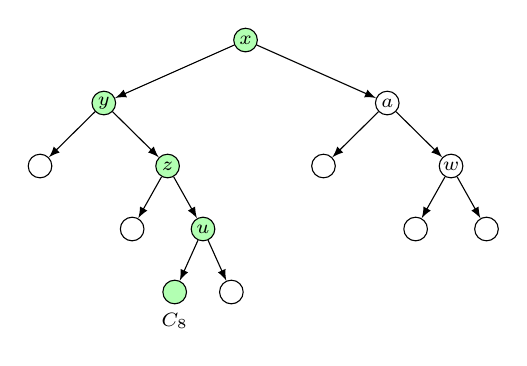
\begin{tikzpicture}[>=latex, xscale = 0.9]
    
    \node[inner, fill = green!30] (a) at (0, 0) {\scriptsize $x$};
    \node[inner, fill = green!30] (b) at (-2, -0.8) {\scriptsize $y$};
    \node[inner] (c) at (2, -0.8) {\scriptsize $a$};
    \node[inner] (d) at (-2.9, -1.6) {};
    \node[inner, fill = green!30] (e) at (-1.1, -1.6) {\scriptsize $z$};
    \node[inner] (f) at (1.1, -1.6) {};
    \node[inner] (g) at (2.9, -1.6) {\scriptsize $w$};

    \node[inner] (h) at (-1.6, -2.4) {};
	\node[inner, fill = green!30] (i) at (-0.6, -2.4) {\scriptsize $u$};
    
    \node[inner] (j) at (2.4, -2.4) {};
    \node[inner] (k) at (3.4, -2.4) {};

    \node[inner, fill = green!30] (l) at (-1, -3.2) {};
    \node[below = 4pt] at (l) {\scriptsize $C_{8}$};
    \node[inner] (m) at (-0.2, -3.2) {};
    
    \draw[ed] (a) -- (b);
    \draw[ed] (a) -- (c);
    \draw[ed] (b) -- (d);
    \draw[ed] (b) -- (e);
    \draw[ed] (c) -- (f);
    \draw[ed] (c) -- (g);
    \draw[ed] (e) -- (h);
    \draw[ed] (e) -- (i);
    \draw[ed] (g) -- (j);
    \draw[ed] (g) -- (k);
    \draw[ed] (i) -- (l);
    \draw[ed] (i) -- (m);
\end{tikzpicture}
    \end{minipage}
    \pause
    \begin{minipage}{0.4\linewidth}
        \centering
        $\frac{A \lor x ~~~ B \lor \neg x}{A \lor B} ~~~~~ \frac{A}{A \lor z}$
        \begin{itemize}
            \item Node $\Rightarrow$ disjunction of negations of queries.
            \item $(x \lor \neg y \lor \neg z \lor u)$.
        \end{itemize}
    \end{minipage}

\end{frame}

\begin{frame}{Corollaries}

    \begin{itemize}
        \item{} Running time of $\DPLL$ on $\PHP_{n}^{n + 1}$ is at least $2^{\Omega(n)}$.
            \pause
        \item{} [Alekhnovich, Hirsch, Itsykson 05; \alert{informal}] Running time of \alert{restricted}
            $\DPLL$ on some \alert{sat. formulas} is at least $2^{\Omega(n)}$. 
    \end{itemize}

    \pause
    \vspace{0.5cm}
    \begin{block}{Remark}
        $\alg{CDCL} \approx$ general resolution.
    \end{block}

    \pause
    \begin{itemize}
        \item{} Running time of $\alg{CDCL}$ on $\PHP_{n}^{n + 1}$ is at least $2^{\Omega(n)}$.
        \item{} \alert{Open problem}: what about sat. formulas and $\alg{CDCL}$?
    \end{itemize}

\end{frame}
    
    \end{center}

    \vspace{0.1cm}
        
	\pause
    \pause
    \pause
    \pause

    Can we estimate running time of this algorithm?

\end{frame}

\begin{frame}{Canonical search problem $\Search_{\varphi}$ (Lov{\'{a}}sz et al. 1994)}
    
    $\varphi(x, y)$ is an unsatisfiable CNF formula:
    \begin{itemize}
        \item Alice receives an assignment to the variables $x$, Bob receives an assignment to the
            variables $y$;
        \item goal is to find a clause $C \in \varphi$ that is unsatisfied by this assignment.
    \end{itemize}

    \pause

    \begin{block}{Beame, Pitassi, Segerlind 06; Huynh, Nordstr{\"{o}}m 12; G{\"{o}}{\"{o}}s, Pitassi 14}
        There is a CNF formula $\varphi$ on $n$ variables such that:
        $$\RCC(\Search_{\varphi}) \ge \RCC(\Disj_{\frac{n}{\log n}}) = \Omega\left( \frac{n}{\log n} \right).$$
    \end{block}

    \begin{block}{Lov{\'{a}}sz et al. 1994}
        Running time of $\DPLL$ on formula $\varphi$ algorithm is at least $2^{\DCC(\Search_{\varphi})}$.
    \end{block}
\end{frame}

\begin{frame}{Lower bound on $\DPLL$}

    \begin{block}{Lov{\'{a}}sz et al. 1994}
        Running time of $\DPLL$ on formula $\varphi$ algorithm is at least $2^{\DCC(\Search_{\varphi})}$.
    \end{block}

    \begin{minipage}{0.54\linewidth}
        \begin{enumerate}
            \item<2-> Pick a subtree $T'$ such that: $\frac{1}{3}|T| \le |T'| \le \frac{1}{3}|T|$.
            \item<4-> Check whether we reach this subtree. Two bits of communication.
            \item<6-> If ``yes'', run algorithm for $T'$.
            \item<7-> If ``no'', run algorithm for $T \setminus T'$.
        \end{enumerate}
    \end{minipage}
    \begin{minipage}{0.45\linewidth}
        \begin{center}
            \tikzstyle{subtree} = [opacity = 0]
\only<3->{\tikzstyle{subtree} = [opacity = 1]}

\tikzstyle{norm} = [semithick, draw = black]
\tikzstyle{acedge} = [black]
\only<5-7>{
    \tikzstyle{acedge} = [
        draw = LEIorange!80, 
        ultra thick]
}


\tikzstyle{end} = [draw, circle, minimum size = 0.6cm, inner sep = 0.1pt]

            
\tikzstyle{level 1} = [level distance = 1.5cm, sibling distance = 2.5cm]
\tikzstyle{level 2} = [sibling distance = 1.5cm]
\tikzstyle{level 3} = [sibling distance = 1.5cm]
    
\begin{tikzpicture}[label distance = 8mm]
    \node[end, acedge] (z) at (0, 0) {$\varphi$}
        child[end]{
            node[end, acedge] {$\varphi'$}
            child[end]{
                node {$\vdots$}
                edge from parent[norm]
	  	        node[above left] {$w \coloneqq 0$}
            }
		    child[end]{
            	node[end] (o) {$\varphi''$}
            	child[end]{
            	   	node {$\vdots$}
            		edge from parent[norm]
	  	        	node[above left] (a) {$y \coloneqq 0$}
                }
                child[end]{
            	   	node {$\vdots$}
            		edge from parent[norm]
	  	        	node[above right] (b) {$y \coloneqq 1$}
            	}
                edge from parent
                node[above right, black] {$w \coloneqq 1$}
            }
           	edge from parent[acedge]
            node[above left, black] {$x \coloneqq 0$}
        }
        child[end]{
            node[end] (c) {$\varphi'''$}
            child[end]{
               	node {$\vdots$}
                edge from parent[norm]
	            node[above left] {$z \coloneqq 0$}
            }
		    child[end]{
               	node {$\vdots$}
                edge from parent[norm]
	            node[above right] {$z \coloneqq 1$}
            }
            edge from parent[norm]
	   	    node[above right] {$x \coloneqq 1$}
        };

        \begin{scope}[on background layer]
            \draw[subtree, ultra thick, orange!25, fill = orange!10, rounded corners = 0.8cm]
                ($(a) + (225:2.12)$) -- ($(o) + (0, 1)$) --
                ($(b) + (-45:2.12)$) node[shift = {(-0.8, 0.3)}, black] {$T'$} -- cycle;
        \end{scope}
\end{tikzpicture}
        \end{center}
    \end{minipage}

    \vspace{0.1cm}
        
	\pause
    \pause
    \pause
    \pause
    \pause
    \pause
    \pause
    
    \vspace{0.1cm}

    We need at most $\log |T|$ recursive calls.

\end{frame}